\section{Partitionnement �tendu: Formater les partitions}
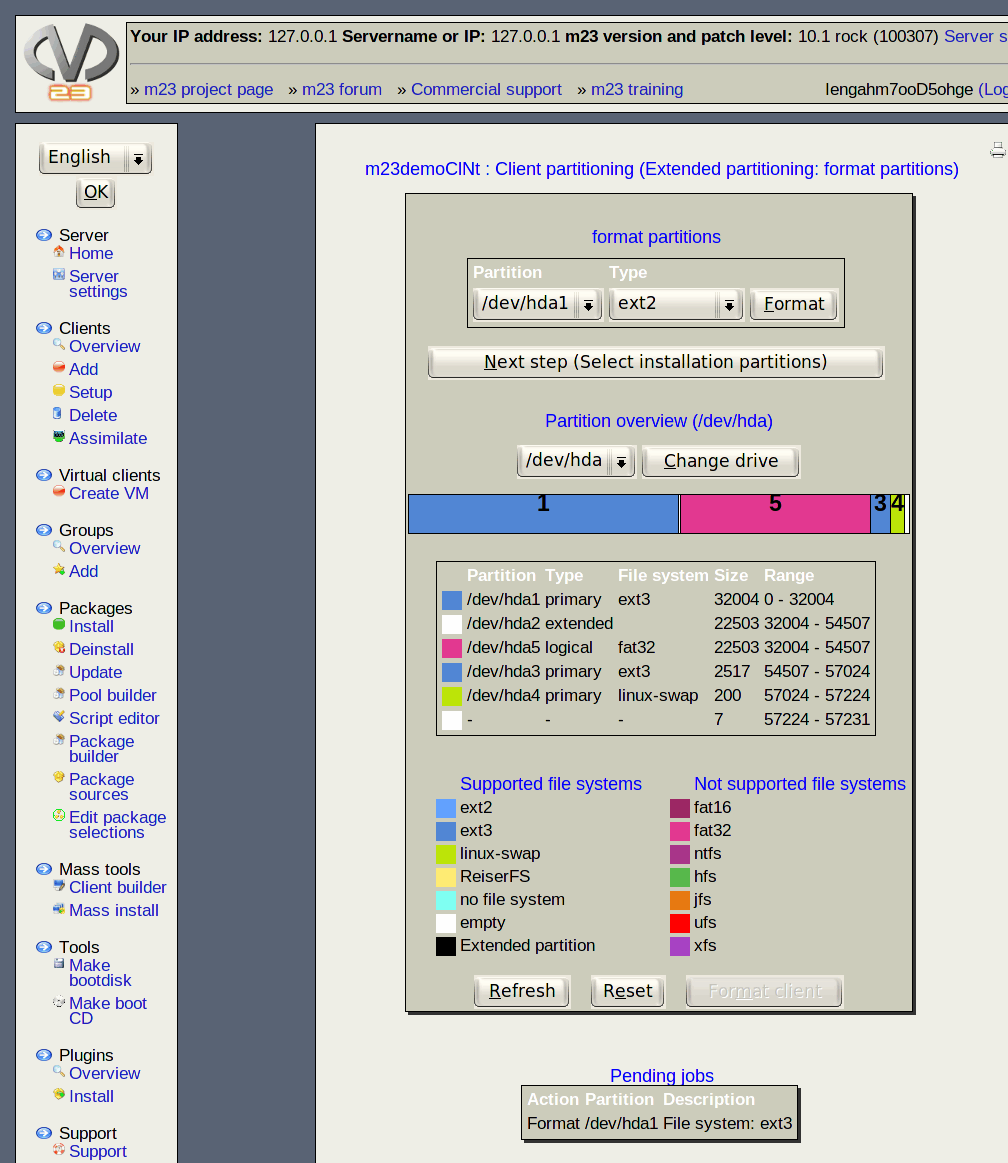
\includegraphics[scale=0.4]{/mdk/doc/manual/screenshots/fr/fdisk-extended2.png} \\
\begin{itemize}
\item Choisissez la partition que vous voudriez formater en s\'electionnant le type du syst\`eme de fichier et cliquant sur \textit{$\ll$Formater$\gg$}. Quant au choix du syst\`eme de fichier $\ll$correct$\gg$, regardez l'information en bas de cette page.\\
\item Quand vous avez format\'e toutes les partitions souhait\'es, cliquez sur \textit{$\ll$$\gg$}.\\
\end{itemize}
\subsection{Information suppl\'ementaire}
Il faut au moins une partition format\'e ext2, ext3 ou reiserfs et une partition avec un syst\`eme de fichier linux-swap pour pouvoir commencer avec l'installation.\\
\subsection{Information: Syst\`emes de fichier}
\begin{itemize}
\item \textbf{ext2:} un syst\`eme de fichier plus \^ag\'e, apte \`a l'installation du syst\`eme de base\\
\item \textbf{ext3(recommand\'e), reiserfs:} syst\`emes de fichier journalling plus modernes, qui sont aptes \`a l'installation du syst\`eme de base \\
\item \textbf{linux-swap:} est utilis\'e pour l'\'etablissement de la m\'emoire linux-swap\\
\end{itemize}
